%===============================================================================
\section{Results}
%===============================================================================
\subsection{Radiation Hydrodynamics MMS Problems}
%-------------------------------------------------------------------------------
To test the full radiation-hydrodynamics system, an MMS (Method of Manufactured
Solutions) problem was designed. The original system given by Equations
\eqref{eq:cons_mass} through \eqref{eq:cons_energy} and \eqref{eq:S2Q} is
the following:
\[
   \dxdy{\rho}{t}+\dxdy{}{x}\fn{\rho u} = 0 \pec
\] 
\[
   \dxdy{}{t}\fn{\rho u} + \dxdy{}{x}\fn{\rho u^2} + \dxdy{}{x}\fn{p}
     = \frac{\sigma_t}{c} \F_0 \pec
\]
\[
   \dxdy{E}{t} + \dxdy{}{x}\bracket{\fn{E+p}u}=-\sigma_a c \fn{aT^4 - \E}
     + \frac{\sigma_t u}{c} \F_0 \pec
\]
\[
  \frac{1}{c}\dydt{\Psi^\pm} + \mu^\pm\dydx{\Psi^\pm} + \sigma_t\Psi^\pm
  = \frac{\sigma_s}{2}\phi + \Q^\pm \pep
\]
To execute an MMS problem, extraneous source terms are added to the
system as follows:
\begin{subequations}
\begin{equation}
   \dxdy{\rho}{t}+\dxdy{}{x}\fn{\rho u} = Q^{ext,\rho} \pec
\end{equation} 
\begin{equation}
   \dxdy{}{t}\fn{\rho u} + \dxdy{}{x}\fn{\rho u^2} + \dxdy{}{x}\fn{p}
     = \frac{\sigma_t}{c} \F_0 + Q^{ext,\rho u} \pec
\end{equation}
\begin{equation}
   \dxdy{E}{t} + \dxdy{}{x}\bracket{\fn{E+p}u}=-\sigma_a c \fn{aT^4 - \E}
     + \frac{\sigma_t u}{c} \F_0 + Q^{ext,E} \pec
\end{equation}
\begin{equation}
  \frac{1}{c}\dydt{\Psi^\pm} + \mu^\pm\dydx{\Psi^\pm} + \sigma_t\Psi^\pm
  = \frac{\sigma_s}{2}\phi + \Q^\pm + Q^{ext,\pm} \pep
\end{equation}
\end{subequations}
Two MMS problems, one for the streaming limit and one for the equilibrium
diffusion limit, were taken from \cite{mcclarren2}.

For the diffusion limit problem, the following solutions were prescribed
for the hydrodynamic solution:
\begin{subequations}
\begin{equation}
  \rho = A\left(\sin(Bx - Ct) + 2\right) \pec
\end{equation}
\begin{equation}
  u = A\left(\cos(Bx - Ct) + 2\right) \pec
\end{equation}
\begin{equation}
  p = A\alpha\left(\cos(Bx - Ct) + 2\right) \pec
\end{equation}
\end{subequations}
where $A$, $B$, and $C$ are constants to be chosen.
As stated in \cite{mcclarren2}, the radiation energy density and flux
are the following in the equilibrium diffusion limit:
\begin{subequations}
\begin{equation}
  \E = T^4 \pec
\end{equation}
\begin{equation}
  \F = \frac{1}{3\sigma}\partial_x T^4 + \frac{4}{3}\frac{u}{\mathbb{C}}T^4 \pec
\end{equation}
\end{subequations}
where $\mathbb{C}$ is a non-dimensional parameter.
Using the ideal gas equation of state relations, an expression
for temperature $T$ can be derived and substituted into these equations,
using a specific heat $c_v$ such that
\begin{equation}
  T = \frac{\gamma p}{\rho} \pep
\end{equation}
Symbolic manipulation can be used to derive the MMS sources
$Q^\rho$, $Q^{\rho u}$, $Q^E$, and $Q^{\pm}$; the resulting expressions
are omitted here due to their complexity and length. The values chosen
for the constants/non-dimensional parameters are $A=B=C=1$, $\alpha=0.5$,
$\gamma=\frac{5}{3}$, and $\mathbb{C}=\sigma=1000$.
Figure \ref{fig:MMS_diffusion_limit_solution} compares the computed hydrodynamic
solutions with the exact solutions for this problem,
and Figure \ref{fig:MMS_diffusion_limit_convergence} shows
that 2nd-order convergence is achieved
(shown here for internal energy).

\begin{figure}[ht]
   \centering
   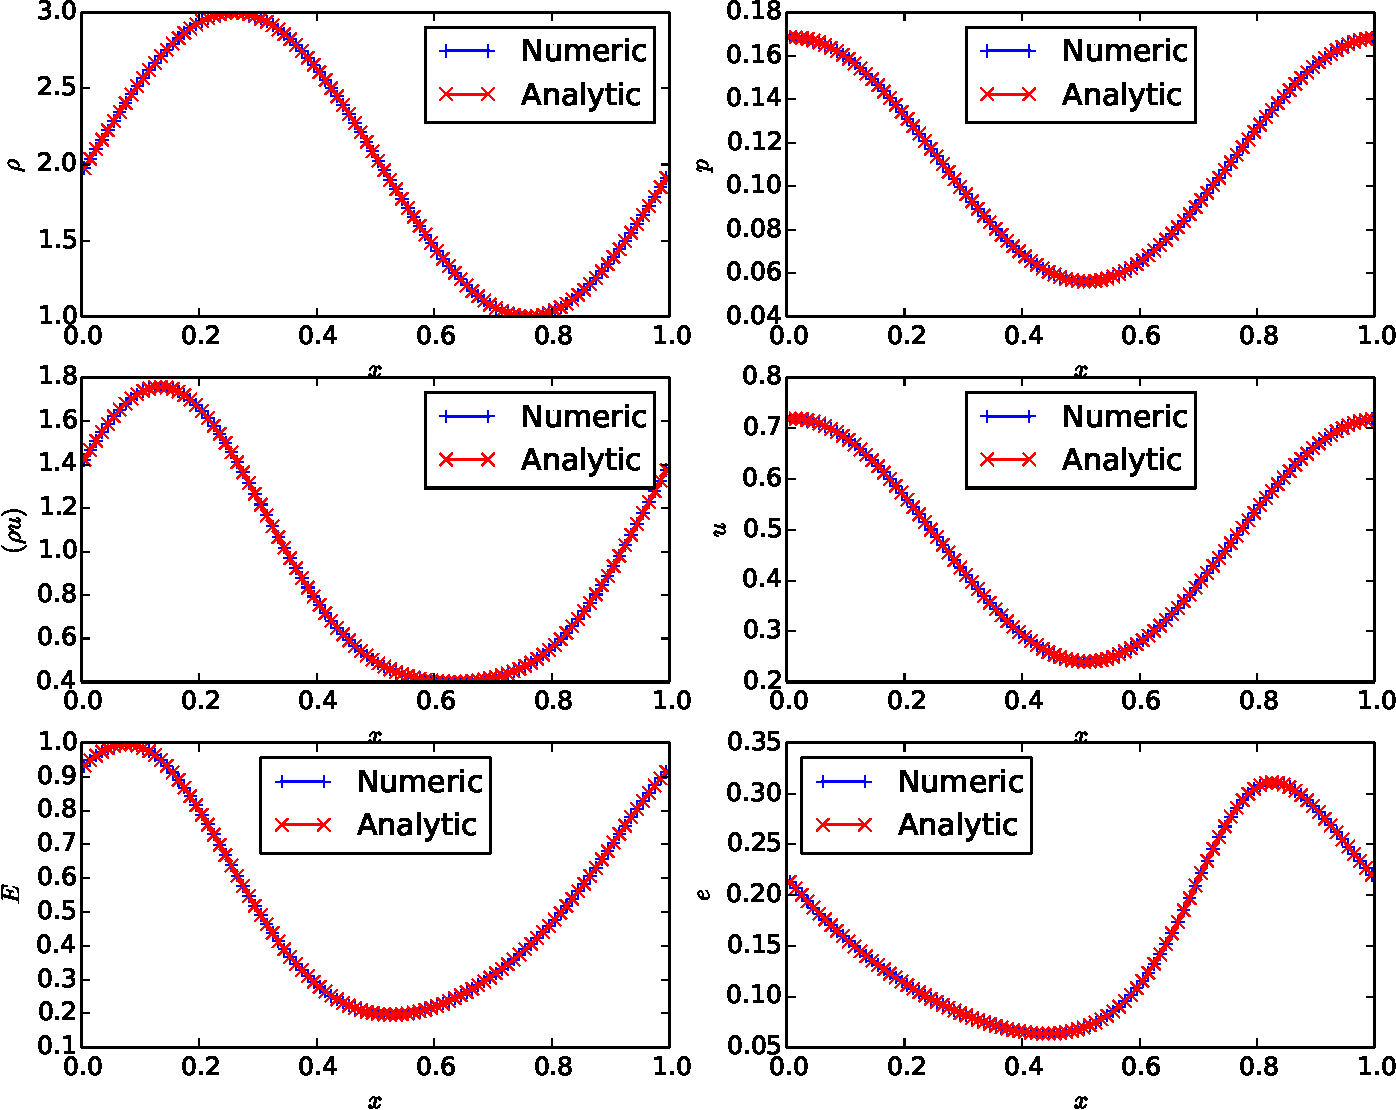
\includegraphics[width=\textwidth]{figures/MMS_diffusion_limit_solution.pdf}
   \caption{Hydrodynamic solution for the equilibrium diffusion limit MMS problem}
   \label{fig:MMS_diffusion_limit_solution}
\end{figure}

\begin{figure}[ht]
   \centering
   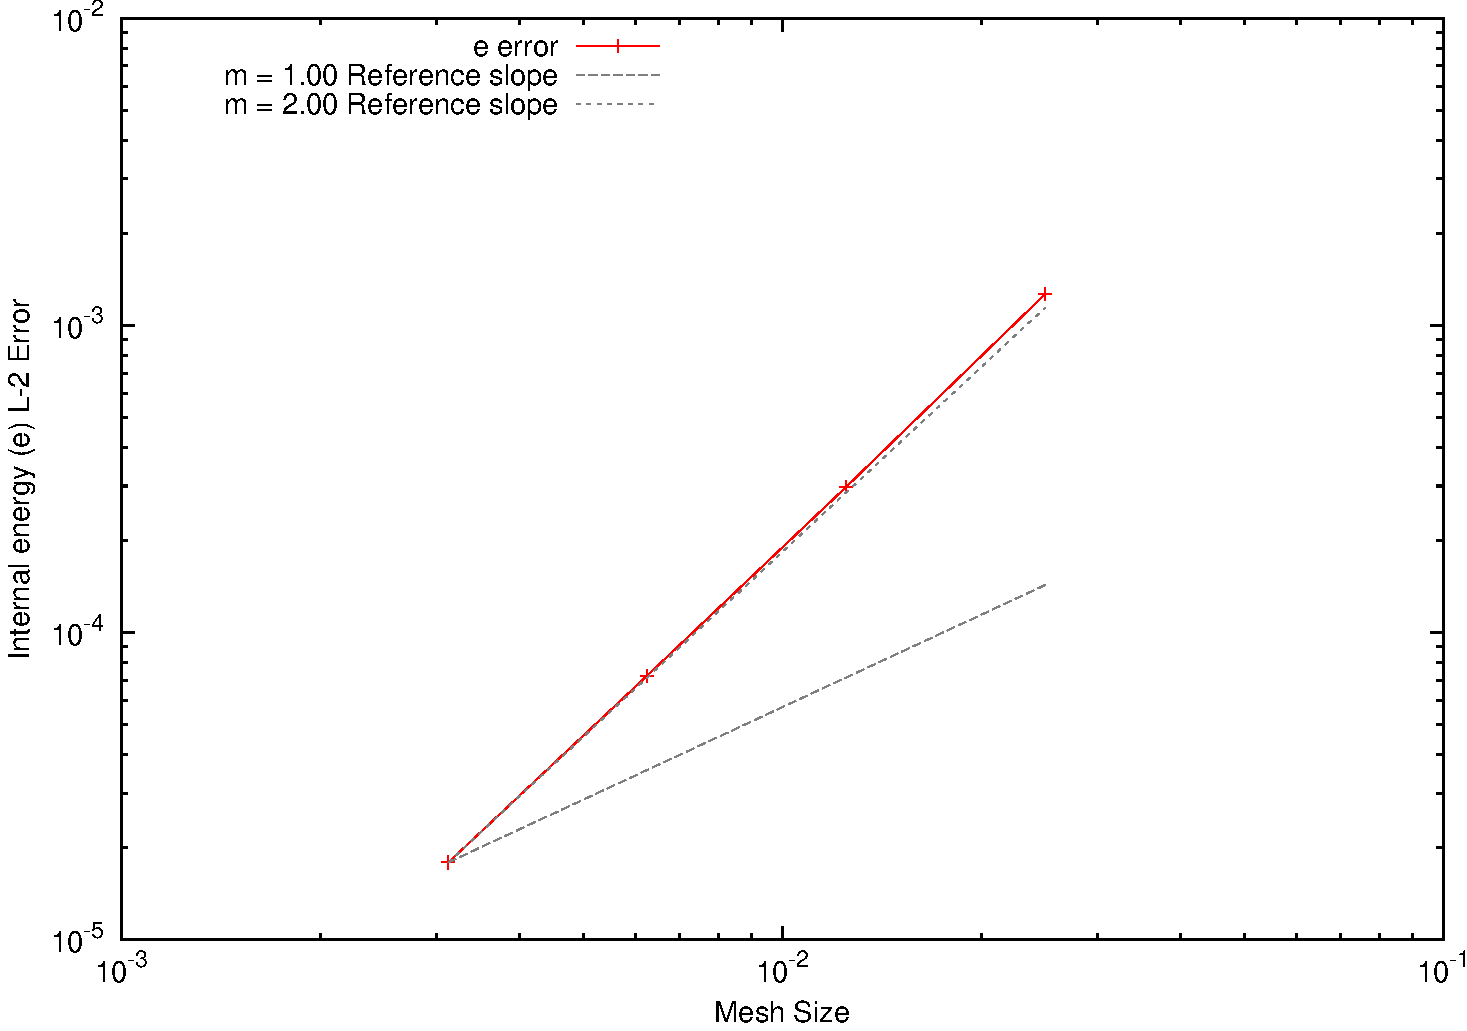
\includegraphics[width=\textwidth]{figures/MMS_diffusion_limit_convergence.pdf}
   \caption{Convergence of internal energy for the equilibrium diffusion limit MMS problem}
   \label{fig:MMS_diffusion_limit_convergence}
\end{figure}

The second MMS problem corresponds to the streaming limit, in which the radiation
and hydrodynamics are weakly coupled due to the high radiation energy propagation
speed relative to the fluid speed. For this problem, the following MMS solutions
are chosen:

%\begin{subequations}
%\end{subequations}

\subsection{Radiation-Hydrodyamics Shocks}
%-------------------------------------------------------------------------------
A Mach 2 radiative shock problem was taken from \cite{edwardsthesis}.
The material properties are uniform and are given in Table
\ref{tab:mach2_shock_material}. Initial conditions in the pre-shock
and post-shock regions are given in Table \ref{tab:mach2_shock_IC}.
Figure \ref{fig:mach2_shock_T} shows the numerical solution computed
with 300 cells and a CFL of 0.6, using the van Leer slope limiter;
the comparison to the reference solution shows excellent agreement.

\begin{table}[ht]
  \centering
  \caption{Material property values for the Mach 2 radiative shock problem}
  \label{tab:mach2_shock_material}
  \begin{tabular}{l l}\hline
    \emph{Parameter} & \emph{Value}\\\hline
    $\sigma_a$ & 390.71164263502112\\
    $\sigma_t$ & 853.14410158161809\\
    $c_v$      & 0.12348\\\hline
  \end{tabular}
\end{table}

\begin{table}[ht]
  \centering
  \caption{Initial condition values for the Mach 2 radiative shock problem}
  \label{tab:mach2_shock_IC}
  \begin{tabular}{l l l}\hline
    \emph{Parameter} & \emph{Pre-shock Value} & \emph{Post-shock Value}\\\hline
    $\rho$           & 1                      & 2.2860748989303659\\
    $u$              & 0.23426480742954117    & 0.10247468599526272\\
    $E$              & 3.9788000000000004e-2  & 7.0649692950433357e-2\\
    $\E$             & 1.3720000000000002e-6  & 2.5560936967521927e-5\\
    $\F$             & 0                      & 0\\\hline
  \end{tabular}
\end{table}

\begin{figure}[ht]
   \centering
   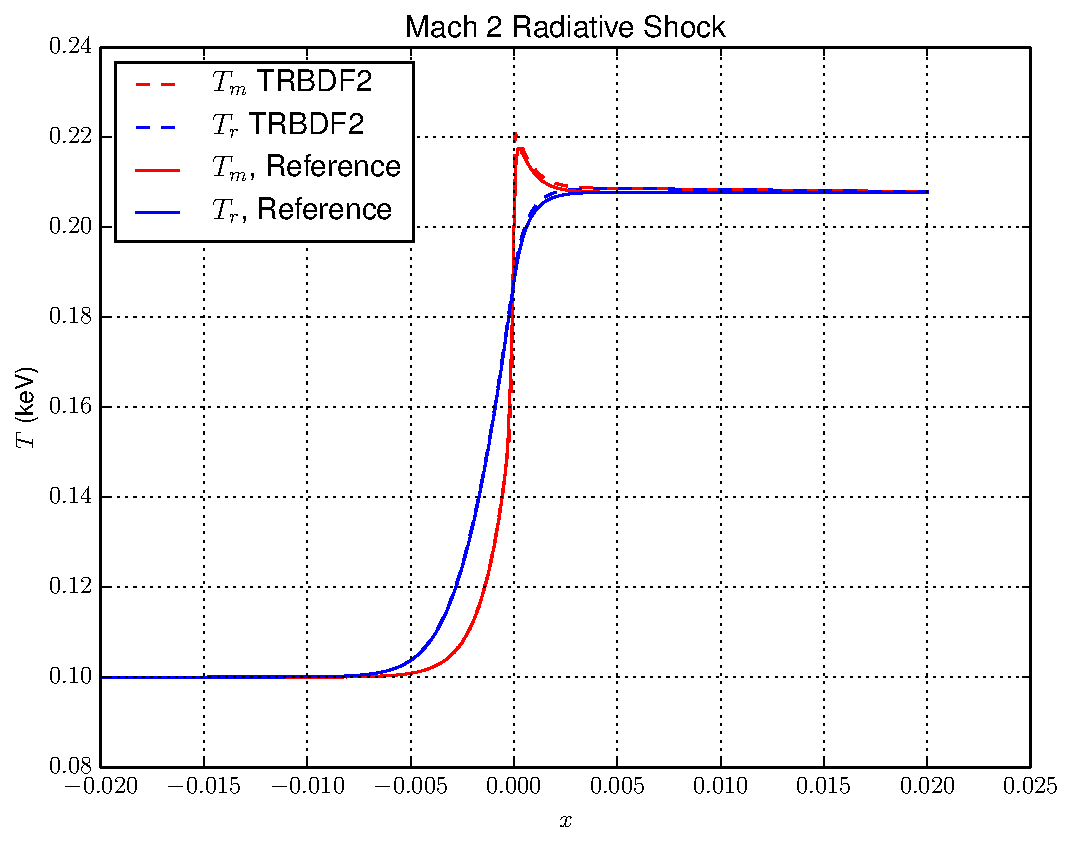
\includegraphics[width=\textwidth]{figures/mach2_shock_T.pdf}
   \caption{Comparison of Mach 2 radiative shock solution to reference solution}
   \label{fig:mach2_shock_T}
\end{figure}

